Most of the braille display products available in the market right now, such as those sold by HumanWare and RNIB, are based on piezoelectric bimorph benders or relay-lever mechanisms.  

The biomorph benders mechanism, shown in figure \ref{fig:piezo-bender} produces vibrations that move the pin up and down when placed in an electric field.
In relay-lever mechanisms, shown in figure \ref{fig:piezo-relay}, when voltage is supplied, the relay pushes the pin up. When the power is off, the weight of the lever mechanism moves the pin downwards to its original position \cite{hernandez_characterization_2009}.

The main drawback of these two popular mechanisms is that benders and relay-lever systems are implemented as an additional burdensome module attached to the contact pins that may compromise integration capacity. According to 
\cite{di_bucchianico_survey_2018}, a typical cell of biomorph piezoelectric braille display has a length of 40mm, and a commercial solution from Johnson Matthey has a length of 60mm for their $4 \times 8$ module \cite{JM_braille_display}, this means that a large space must be left between lines of cells in order for the biomorph bender to function properly. In addition to that, the weight of current commercial braille display are usually ranging from 400g to 1kg \cite{Humanware_BrailleNote} \cite{Brailliant_BI_40X}.
In consequence, Braille displays are not usually portable. Besides, the common cost for a single piezoelectric cells about USD 100 to the end user \cite{runyan_eap_2010}, setting the price of even single line refreshable braille display (RBD) well over USD 1000. The small size of the market also limits the incentive of bringing these prices down.

\begin{figure}[ht] \centering
    \begin{subfigure}[b]{0.4\textwidth}\centering
        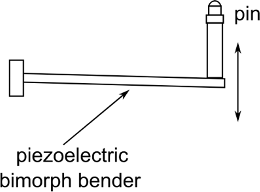
\includegraphics[height=3cm]{figures/piezo-bender-a.png}
        \caption{}
        \label{fig:piezo-bender}
    \end{subfigure}
    \begin{subfigure}[b]{0.4\textwidth}\centering
        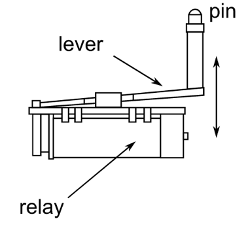
\includegraphics[height=3.5cm]{figures/piezo-bender-b.png}
        \caption{}
        \label{fig:piezo-relay}
    \end{subfigure}
\caption[Examples of existing Braille mechanisms]{Examples of existing Braille mechanisms: (a) piezoelectric bimorph bender and (b) relay-lever system \cite{hernandez_characterization_2009}. Despite their popularity, high cost and dimensions make it unsuitable for a 2D refreshable braille display.}
\label{fig:piezo-bender-schema}
\end{figure}

Another recently developed mechanism is piezoelectric ultrasonic motor \cite{hernandez_characterization_2009}.
The ultrasonic linear motor consists of a shaft, a mobile element or slider, and a piezoelectric ceramic disk as shown in figure \ref{fig:piezo-miniature-a}.
The key advantage of this design is the ultra-light weight of this miniature motor.
However, the need for several layers, shown in figure \ref{fig:piezo-miniature-b}, does not befit the density required by a 2D tactile display.

\begin{figure}[ht] \centering
    \begin{subfigure}[b]{0.45\textwidth}\centering
        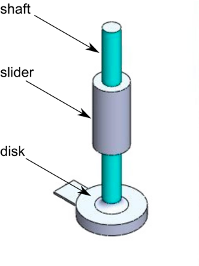
\includegraphics[height=5cm]{figures/piezo-miniature-a.png}
        \caption{}
        \label{fig:piezo-miniature-a}
    \end{subfigure}
    \begin{subfigure}[b]{0.50\textwidth}\centering
        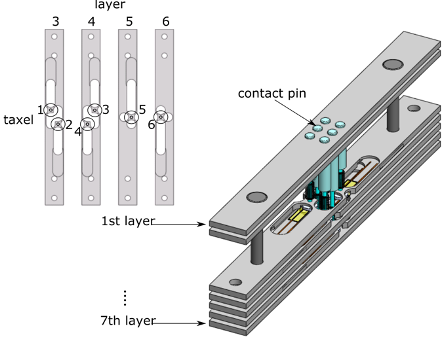
\includegraphics[height=6cm]{figures/piezo-full-design-a.png}
        \caption{}
        \label{fig:piezo-miniature-b}
    \end{subfigure}
\caption[Miniature piezoelectric linear motor]{Miniature ultrasonic piezoelectric linear motor: (a) conceptual design and (b) in-situ. Despite its low weight, the requirement of several layers to create one cell makes it unviable for the density required by a 2D display.}
\label{fig:piezo-miniature}
\end{figure}